% answers.tex —— 2005 年·普通高等学校招生考试·湖北卷·理科 · 参考答案与详细解析片段
% 由 tools/generate_projects.py 依来源总账自 2005/2005_数学真题_湖北理科_试题.md + 2005/2005_数学真题_湖北理科_解析正文.md + 2005/2005_数学真题_湖北理科_答案要点.md 生成，勿手改（改源 MD 后重跑）

\begin{answer}
\gksolhead{1}{}

\textbf{题目}：

设 $P$、$Q$ 为两个非空实数集合，定义集合 $P + Q = \{a + b \mid a \in P, b \in Q\}$，若 $P = \{0, 2, 5\}, Q = \{1, 2, 6\}$，则 $P + Q$ 中元素的个数是\mbox{（　　）}

\begin{gkopts}(4)
\task A．9
\task B．8
\task C．7
\task D．6
\end{gkopts}

\Needspace{4\baselineskip}
\textbf{解析}

根据题意，集合 $P + Q$ 中的元素由 $a \in P$ 与 $b \in Q$ 的所有可能和构成：
\begin{itemize}
\item 取 $a = 0$ 时：$0 + 1 = 1$，$0 + 2 = 2$，$0 + 6 = 6$；
\item 取 $a = 2$ 时：$2 + 1 = 3$，$2 + 2 = 4$，$2 + 6 = 8$；
\item 取 $a = 5$ 时：$5 + 1 = 6$（已存在），$5 + 2 = 7$，$5 + 6 = 11$．
\end{itemize}

\Needspace{5\baselineskip}
综合去重后得到集合：
\nopagebreak[4]
\[
P + Q = \{1, 2, 3, 4, 6, 7, 8, 11\}.
\]
元素个数共有 8 个．

故选 B．

\gkanswer{答案：B}

\end{answer}
\begin{answer}
\gksolhead{2}{}

\textbf{题目}：

对任意实数 $a, b, c$，给出下列命题：

① “$a = b$”是“$ac = bc$”充要条件；

② “$a + 5$ 是无理数”是“$a$ 是无理数”的充要条件；

③ “$a > b$”是“$a^2 > b^2$”的充分条件；

④ “$a < 5$”是“$a < 3$”的必要条件．

其中真命题的个数是\mbox{（　　）}

\begin{gkopts}(4)
\task A．1
\task B．2
\task C．3
\task D．4
\end{gkopts}

\Needspace{4\baselineskip}
\textbf{解析}

逐一分析各命题的真假：
\begin{itemize}
\item 对于 ①：若 $c = 0$，由 $ac = bc$ 不能推得 $a = b$，故“$a = b$”是“$ac = bc$”的充分不必要条件，① 为假命题；
\item 对于 ②：若 $a$ 为无理数，假设 $a + 5 = r \in \mathbf{Q}$，则 $a = r - 5 \in \mathbf{Q}$，矛盾，故 $a + 5$ 必为无理数；反之，若 $a + 5$ 为无理数，假设 $a = r \in \mathbf{Q}$，则 $a + 5 = r + 5 \in \mathbf{Q}$，亦矛盾，故 $a$ 必为无理数．因此“$a + 5$ 是无理数”是“$a$ 是无理数”的充要条件，② 为真命题；
\item 对于 ③：取 $a = 1, b = -2$，满足 $a > b$，但 $a^2 = 1 < b^2 = 4$，充分性不成立，③ 为假命题；
\item 对于 ④：若 $a < 3$，则显然满足 $a < 5$，即 $(-\infty, 3) \subset (-\infty, 5)$，因此“$a < 5$”是“$a < 3$”的必要条件，④ 为真命题．
\end{itemize}

综上，真命题共有 ②、④ 两个．

故选 B．

\gkanswer{答案：B}

\end{answer}
\begin{answer}
\gksolhead{3}{}

\textbf{题目}：

函数 $y = \mathrm{e}^{|\ln x|} - |x - 1|$ 的图象大致是\mbox{（　　）}
\nopagebreak[4]
\begin{center}% 2005 年湖北卷理科第 3 题选项图：函数 y = e^{|\ln x|} - |x-1| 的图象 4 个选项
\begin{tikzpicture}[>=stealth,scale=0.9,line cap=round]
  % (A)
  \begin{scope}
    \draw[->] (-0.8,0) -- (2.6,0) node[below] {$x$};
    \draw[->] (0,-0.8) -- (0,2.6) node[left] {$y$};
    \node[below left] at (0,0) {$O$};
    \draw (1,0.08) -- (1,-0.08) node[below] {$1$};
    \draw (0.08,1) -- (-0.08,1) node[left] {$1$};
    \draw[thick] (0.06,1) -- (2.2,1);
    \draw[fill=white] (0,1) circle (1.5pt);
    \node at (-0.6,-1.1) {(A)};
  \end{scope}

  % (B)
  \begin{scope}[xshift=5.8cm]
    \draw[->] (-0.8,0) -- (2.6,0) node[below] {$x$};
    \draw[->] (0,-0.8) -- (0,2.6) node[left] {$y$};
    \node[below left] at (0,0) {$O$};
    \draw (1,0.08) -- (1,-0.08) node[below left] {$1$};
    \draw (0.08,1) -- (-0.08,1) node[left] {$1$};
    \draw[thick] (1,1) -- (2.2,1);
    \draw[dashed] (1,0) -- (1,1);
    \draw[dashed] (0,1) -- (1,1);
    \draw[dashed] (1,0) -- (1,0.4);
    \draw[thick,domain=0.35:0.96,samples=30] plot (\x,{0.4*sqrt(\x) + 0.8*(\x-1)});
    \draw[fill=white] (1,0.4) circle (1.5pt);
    \node at (-0.6,-1.1) {(B)};
  \end{scope}

  % (C)
  \begin{scope}[yshift=-4.8cm]
    \draw[->] (-0.8,0) -- (2.6,0) node[below] {$x$};
    \draw[->] (0,-0.8) -- (0,2.6) node[left] {$y$};
    \node[below left] at (0,0) {$O$};
    \draw (1,0.08) -- (1,-0.08) node[below] {$1$};
    \draw (0.08,1) -- (-0.08,1) node[left] {$1$};
    \draw[dashed] (1,0) -- (1,1);
    \draw[dashed] (0,1) -- (1,1);
    \draw[thick,domain=0.35:1,samples=30] plot (\x,{\x + 1/\x - 1});
    \draw[thick] (1,1) -- (2.0,2.0);
    \node at (-0.6,-1.1) {(C)};
  \end{scope}

  % (D) 正确选项
  \begin{scope}[xshift=5.8cm,yshift=-4.8cm]
    \draw[->] (-0.8,0) -- (2.6,0) node[below] {$x$};
    \draw[->] (0,-0.8) -- (0,2.6) node[left] {$y$};
    \node[below left] at (0,0) {$O$};
    \draw (1,0.08) -- (1,-0.08) node[below] {$1$};
    \draw (0.08,1) -- (-0.08,1) node[left] {$1$};
    \draw[dashed] (1,0) -- (1,1);
    \draw[dashed] (0,1) -- (1,1);
    \draw[thick,domain=0.35:1,samples=40] plot (\x,{\x + 1/\x - 1});
    \draw[thick] (1,1) -- (2.2,1);
    \node at (-0.6,-1.1) {(D)};
  \end{scope}
\end{tikzpicture}
\end{center}
\nopagebreak[4]
\begin{gkopts}(1)
\task A．在 $x > 0$ 上恒等于 1 的水平射线（不含点 $(0, 1)$）
\task B．在 $(0, 1)$ 上递增、在 $[1, +\infty)$ 上恒等于 1 的图象
\task C．在 $(0, 1)$ 上递减、在 $[1, +\infty)$ 上斜向上递增的折线
\task D．在 $(0, 1)$ 上为下凸递减曲线、在 $[1, +\infty)$ 上为水平射线 $y = 1$ 的图象
\end{gkopts}

\Needspace{4\baselineskip}
\textbf{解析}

化简函数解析式：
定义域为 $x \in (0, +\infty)$．
\begin{itemize}
\item 当 $0 < x < 1$ 时，$|\ln x| = -\ln x$，$\mathrm{e}^{|\ln x|} = \mathrm{e}^{-\ln x} = \dfrac{1}{x}$；
\end{itemize}
\Needspace{5\baselineskip}
  又 $|x - 1| = 1 - x$，故：
\nopagebreak[4]
\[
y = \frac{1}{x} - (1 - x) = x + \frac{1}{x} - 1.
\]
  对 $x \in (0, 1)$ 求导：$y' = 1 - \dfrac{1}{x^2} = \dfrac{x^2 - 1}{x^2} < 0$，二阶导数 $y'' = \dfrac{2}{x^3} > 0$．
  因此图象在 $(0, 1)$ 上为严格单调递减的下凸曲线，且当 $x \to 0^+$ 时 $y \to +\infty$，当 $x \to 1^-$ 时 $y \to 1$；
\begin{itemize}
\item 当 $x \geqslant 1$ 时，$|\ln x| = \ln x$，$\mathrm{e}^{|\ln x|} = \mathrm{e}^{\ln x} = x$；
\end{itemize}
\Needspace{5\baselineskip}
  又 $|x - 1| = x - 1$，故：
\nopagebreak[4]
\[
y = x - (x - 1) = 1.
\]
  图象在 $[1, +\infty)$ 上为一条水平射线 $y = 1$．

对照各选项图象特征可知，选项 D 正确．

故选 D．

\gkanswer{答案：D}

\end{answer}
\begin{answer}
\gksolhead{4}{}

\textbf{题目}：

木星的体积约是地球体积的 $240\sqrt{30}$ 倍，则它的表面积约是地球表面积的\mbox{（　　）}

\begin{gkopts}(2)
\task A．60 倍
\task B．$60\sqrt{30}$ 倍
\task C．120 倍
\task D．$120\sqrt{30}$ 倍
\end{gkopts}

\Needspace{4\baselineskip}
\textbf{解析}

设木星与地球的半径分别为 $R_1, R_2$，均视为球体．
\Needspace{5\baselineskip}
由球体体积公式 $V = \dfrac{4}{3}\pi R^3$ 可得：
\nopagebreak[4]
\[
\frac{V_1}{V_2} = \left(\frac{R_1}{R_2}\right)^3 = 240\sqrt{30}.
\]
\Needspace{5\baselineskip}
注意到：
\nopagebreak[4]
\[
240\sqrt{30} = \sqrt{240^2 \times 30} = \sqrt{57600 \times 30} = \sqrt{1728000} = \sqrt{120^3} = 120^{3/2} = (\sqrt{120})^3.
\]
\Needspace{5\baselineskip}
因此半径之比为：
\nopagebreak[4]
\[
\frac{R_1}{R_2} = \sqrt{120}.
\]
\Needspace{5\baselineskip}
由球体表面积公式 $S = 4\pi R^2$ 可得木星与地球表面积之比为：
\nopagebreak[4]
\[
\frac{S_1}{S_2} = \left(\frac{R_1}{R_2}\right)^2 = (\sqrt{120})^2 = 120.
\]
故木星的表面积约是地球表面积的 120 倍．

故选 C．

\gkanswer{答案：C}

\end{answer}
\begin{answer}
\gksolhead{5}{}

\textbf{题目}：

双曲线 $\dfrac{x^2}{m} - \dfrac{y^2}{n} = 1$ ($mn \neq 0$) 离心率为 2，有一个焦点与抛物线 $y^2 = 4x$ 的焦点重合，则 $mn$ 的值为\mbox{（　　）}

\begin{gkopts}(4)
\task A．$\dfrac{3}{16}$
\task B．$\dfrac{3}{8}$
\task C．$\dfrac{16}{3}$
\task D．$\dfrac{8}{3}$
\end{gkopts}

\Needspace{4\baselineskip}
\textbf{解析}

抛物线 $y^2 = 4x$ 的标准形式为 $y^2 = 2px$ ($p = 2$)，其焦点坐标为 $(1, 0)$．
因为双曲线 $\dfrac{x^2}{m} - \dfrac{y^2}{n} = 1$ 的焦点与之重合，所以该双曲线焦点在 $x$ 轴上，焦点坐标为 $(c, 0) = (1, 0)$，即 $c = 1$．
由双曲线方程可知 $a^2 = m > 0$，$b^2 = n > 0$，且 $c^2 = a^2 + b^2 = m + n = 1$．
\Needspace{5\baselineskip}
由离心率公式 $e = \dfrac{c}{a} = 2$，得：
\nopagebreak[4]
\[
a = \frac{c}{2} = \frac{1}{2} \implies m = a^2 = \frac{1}{4}.
\]
\Needspace{5\baselineskip}
进而得到：
\nopagebreak[4]
\[
n = b^2 = c^2 - a^2 = 1 - \frac{1}{4} = \frac{3}{4}.
\]
\Needspace{5\baselineskip}
所以：
\nopagebreak[4]
\[
mn = \frac{1}{4} \times \frac{3}{4} = \frac{3}{16}.
\]

故选 A．

\gkanswer{答案：A}

\end{answer}
\begin{answer}
\gksolhead{6}{}

\textbf{题目}：

在 $y = 2^x, y = \log_2 x, y = x^2, y = \cos 2x$ 这四个函数中，当 $0 < x_1 < x_2 < 1$ 时，使 $f\left(\dfrac{x_1 + x_2}{2}\right) > \dfrac{f(x_1) + f(x_2)}{2}$ 恒成立的函数的个数是\mbox{（　　）}

\begin{gkopts}(4)
\task A．0
\task B．1
\task C．2
\task D．3
\end{gkopts}

\Needspace{4\baselineskip}
\textbf{解析}

不等式 $f\left(\dfrac{x_1 + x_2}{2}\right) > \dfrac{f(x_1) + f(x_2)}{2}$（当 $0 < x_1 < x_2 < 1$ 时恒成立）表示函数在区间 $(0, 1)$ 上为严格上凸（严格凹）函数．若函数二阶可导，充分条件为其二阶导数在 $(0, 1)$ 上恒满足 $f''(x) < 0$．
逐一检验四个函数：
\begin{itemize}
\item 对于 $y = 2^x$：$y' = 2^x \ln 2$，$y'' = 2^x (\ln 2)^2 > 0$，为严格下凸函数，不满足条件；
\item 对于 $y = \log_2 x$：$y' = \dfrac{1}{x\ln 2}$，$y'' = -\dfrac{1}{x^2\ln 2} < 0$，在 $(0, 1)$ 上恒为严格上凸函数，满足条件；
\item 对于 $y = x^2$：$y' = 2x$，$y'' = 2 > 0$，为严格下凸函数，不满足条件；
\item 对于 $y = \cos 2x$：$y' = -2\sin 2x$，$y'' = -4\cos 2x$．当 $x \in (0, 1)$ 时，$2x \in (0, 2)$．在 $\left(0, \dfrac{\pi}{2}\right)$ 上 $\cos 2x > 0 \implies y'' < 0$；而在 $\left(\dfrac{\pi}{2}, 2\right)$ 上 $\cos 2x < 0 \implies y'' > 0$．因此在 $(0, 1)$ 上既有上凸区间又有下凸区间，不能保证对任意 $0 < x_1 < x_2 < 1$ 恒成立．
\end{itemize}

综上所述，满足条件的函数只有 $y = \log_2 x$ 这 1 个．

故选 B．

\gkanswer{答案：B}

\end{answer}
\begin{answer}
\gksolhead{7}{}

\textbf{题目}：

若 $\sin\alpha + \cos\alpha = \tan\alpha$ $\left(0 < \alpha < \dfrac{\pi}{2}\right)$，则 $\alpha \in$\mbox{（　　）}

\begin{gkopts}(2)
\task A．$\left(0, \dfrac{\pi}{6}\right)$
\task B．$\left(\dfrac{\pi}{6}, \dfrac{\pi}{4}\right)$
\task C．$\left(\dfrac{\pi}{4}, \dfrac{\pi}{3}\right)$
\task D．$\left(\dfrac{\pi}{3}, \dfrac{\pi}{2}\right)$
\end{gkopts}

\Needspace{4\baselineskip}
\textbf{解析}

设函数 $f(x) = \sin x + \cos x - \tan x$，$x \in \left(0, \dfrac{\pi}{2}\right)$．
检验各特殊角的值：
\begin{itemize}
\item 当 $x = \dfrac{\pi}{4}$ 时：
\end{itemize}
\nopagebreak[4]
\[
f\left(\frac{\pi}{4}\right) = \sin\frac{\pi}{4} + \cos\frac{\pi}{4} - \tan\frac{\pi}{4} = \frac{\sqrt{2}}{2} + \frac{\sqrt{2}}{2} - 1 = \sqrt{2} - 1 > 0;
\]
\begin{itemize}
\item 当 $x = \dfrac{\pi}{3}$ 时：
\end{itemize}
\nopagebreak[4]
\[
f\left(\frac{\pi}{3}\right) = \sin\frac{\pi}{3} + \cos\frac{\pi}{3} - \tan\frac{\pi}{3} = \frac{\sqrt{3}}{2} + \frac{1}{2} - \sqrt{3} = \frac{1 - \sqrt{3}}{2} < 0.
\]

由零点存在性定理，在连续区间 $\left(\dfrac{\pi}{4}, \dfrac{\pi}{3}\right)$ 内必存在实根．
另一方面：
\begin{itemize}
\item 当 $x \in \left(0, \dfrac{\pi}{4}\right]$ 时，$\tan x \leqslant 1$，而 $\sin x + \cos x = \sqrt{2}\sin\left(x + \dfrac{\pi}{4}\right) > 1$，恒有 $f(x) > 0$，无根；
\item 当 $x \in \left[\dfrac{\pi}{3}, \dfrac{\pi}{2}\right)$ 时，$\tan x \geqslant \sqrt{3} \approx 1.732$，而 $\sin x + \cos x \leqslant \sqrt{2} \approx 1.414$，恒有 $f(x) < 0$，无根．
\end{itemize}

因此方程的根 $\alpha \in \left(\dfrac{\pi}{4}, \dfrac{\pi}{3}\right)$．

故选 C．

\gkanswer{答案：C}

\end{answer}
\begin{answer}
\gksolhead{8}{}

\textbf{题目}：

若 $\lim_{x\to 1} \left(\dfrac{a}{1 - x} - \dfrac{b}{1 - x^2}\right) = 1$，则常数 $a, b$ 的值为\mbox{（　　）}

\begin{gkopts}(4)
\task A．$a = -2, b = 4$
\task B．$a = 2, b = -4$
\task C．$a = -2, b = -4$
\task D．$a = 2, b = 4$
\end{gkopts}

\Needspace{4\baselineskip}
\textbf{解析}

\Needspace{5\baselineskip}
对极限式进行通分整理：
\nopagebreak[4]
\[
\frac{a}{1 - x} - \frac{b}{1 - x^2} = \frac{a(1 + x) - b}{(1 - x)(1 + x)} = \frac{ax + a - b}{1 - x^2}.
\]
当 $x \to 1$ 时，分母 $1 - x^2 \to 0$．
\Needspace{5\baselineskip}
要使极限存在且为有限常数 1，分子在 $x \to 1$ 时的极限必为 0，即：
\nopagebreak[4]
\[
a(1) + a - b = 0 \implies 2a - b = 0 \implies b = 2a.
\]
\Needspace{5\baselineskip}
将 $b = 2a$ 代入分子可得：
\nopagebreak[4]
\[
ax + a - 2a = a(x - 1) = -a(1 - x).
\]
\Needspace{5\baselineskip}
约去公因式 $1 - x$（因 $x \to 1$ 且 $x \neq 1$）：
\nopagebreak[4]
\[
\lim_{x\to 1} \frac{-a(1 - x)}{(1 - x)(1 + x)} = \lim_{x\to 1} \frac{-a}{1 + x} = -\frac{a}{2}.
\]
\Needspace{5\baselineskip}
由题意，极限值为 1，故：
\nopagebreak[4]
\[
-\frac{a}{2} = 1 \implies a = -2.
\]
\Needspace{5\baselineskip}
从而：
\nopagebreak[4]
\[
b = 2a = 2 \times (-2) = -4.
\]

故选 C．

\gkanswer{答案：C}

\end{answer}
\begin{answer}
\gksolhead{9}{}

\textbf{题目}：

若 $0 < x < \dfrac{\pi}{2}$，则 $2^x$ 与 $3\sin x$ 的大小关系\mbox{（　　）}

\begin{gkopts}(2)
\task A．$2^x > 3\sin x$
\task B．$2^x < 3\sin x$
\task C．$2^x = 3\sin x$
\task D．与 $x$ 的取值有关
\end{gkopts}

\Needspace{4\baselineskip}
\textbf{解析}

比较函数 $f(x) = 2^x$ 与 $g(x) = 3\sin x$ 在区间 $\left(0, \dfrac{\pi}{2}\right)$ 上的取值：
\begin{itemize}
\item 当 $x$ 充分接近 0 时，如取 $x \to 0^+$，有 $2^x \to 1$ 而 $3\sin x \to 0$，此时 $2^x > 3\sin x$；
\end{itemize}
  具体而言，若取 $x = \dfrac{1}{10}$，则 $2^{0.1} \approx 1.072$，$3\sin 0.1 \approx 3 \times 0.0998 = 0.2995$，显然 $2^x > 3\sin x$；
\begin{itemize}
\item 若取 $x = \dfrac{\pi}{3}$，则 $2^{\pi/3} \approx 2^{1.047} \approx 2.066$，$3\sin\dfrac{\pi}{3} = \dfrac{3\sqrt{3}}{2} \approx 2.598$，此时 $2^x < 3\sin x$；
\item 若取 $x = \dfrac{\pi}{2}$，则 $2^{\pi/2} \approx 2^{1.57} \approx 2.97$，$3\sin\dfrac{\pi}{2} = 3$，此时 $2^x < 3\sin x$．
\end{itemize}

由此可知，$2^x$ 与 $3\sin x$ 的大小关系取决于自变量 $x$ 的具体取值．

故选 D．

\gkanswer{答案：D}

\end{answer}
\begin{answer}
\gksolhead{10}{}

\textbf{题目}：

如图，在三棱柱 $ABC - A'B'C'$ 中，点 $E, F, H, K$ 分别为 $AC', CB', A'B, B'C'$ 的中点，$G$ 为 $\triangle ABC$ 的重心．从 $K, H, G, B'$ 中取一点作为 $P$，使得该棱柱恰有 2 条棱与平面 $PEF$ 平行，则 $P$ 为\mbox{（　　）}
\nopagebreak[4]
\begin{center}% 2005 年湖北卷理科第 10 题配图：三棱柱 ABC-A'B'C' 与点 E, F, H, K, G
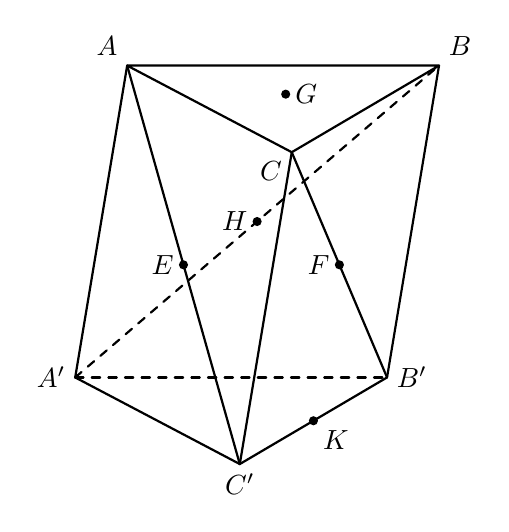
\begin{tikzpicture}[>=stealth,scale=1.1,line cap=round,line join=round]
  % 顶点坐标
  \coordinate (A) at (0,3.0);
  \coordinate (B) at (3.6,3.0);
  \coordinate (C) at (1.9,2.0);
  \coordinate (A1) at (-0.6,-0.6);
  \coordinate (B1) at (3.0,-0.6);
  \coordinate (C1) at (1.3,-1.6);

  % 中点与重心坐标
  \coordinate (G) at (1.83,2.67);
  \coordinate (E) at (0.65,0.7);
  \coordinate (F) at (2.45,0.7);
  \coordinate (H) at (1.5,1.2);
  \coordinate (K) at (2.15,-1.1);

  % 虚线不可见棱与对角线
  \draw[dashed,thick] (A1) -- (B1);
  \draw[dashed,thick] (A1) -- (B);

  % 实线可见棱
  \draw[thick] (A) -- (B) -- (C) -- cycle;
  \draw[thick] (A) -- (A1);
  \draw[thick] (B) -- (B1);
  \draw[thick] (C) -- (C1);
  \draw[thick] (A1) -- (C1) -- (B1);

  % 面对角线
  \draw[thick] (A) -- (C1);
  \draw[thick] (C) -- (B1);

  % 特殊点绘制
  \fill (G) circle (1.5pt) node[right] {$G$};
  \fill (E) circle (1.5pt) node[left] {$E$};
  \fill (F) circle (1.5pt) node[left] {$F$};
  \fill (H) circle (1.5pt) node[left] {$H$};
  \fill (K) circle (1.5pt) node[below right] {$K$};

  % 顶点标签
  \node[above left] at (A) {$A$};
  \node[above right] at (B) {$B$};
  \node[below left] at (C) {$C$};
  \node[left] at (A1) {$A'$};
  \node[right] at (B1) {$B'$};
  \node[below] at (C1) {$C'$};
\end{tikzpicture}
\end{center}
\nopagebreak[4]
\begin{gkopts}(4)
\task A．$K$
\task B．$H$
\task C．$G$
\task D．$B'$
\end{gkopts}

\Needspace{4\baselineskip}
\textbf{解析}

在三棱柱 $ABC - A'B'C'$ 中，侧面均为平行四边形．
因为 $E$ 为对角线 $AC'$ 的中点，在平行四边形 $ACC'A'$ 中对角线互相平分，故 $E$ 亦为 $A'C$ 的中点；
同理，$F$ 为 $CB'$ 的中点，在平行四边形 $BCC'B'$ 中对角线互相平分，故 $F$ 亦为 $BC'$ 的中点．
连接 $AB, A'B'$，用空间向量表示：
\Needspace{5\baselineskip}
设 $\vec{CA} = \vec{a}, \vec{CB} = \vec{b}, \vec{CC'} = \vec{c}$，则：
\nopagebreak[4]
\[
\vec{E} = \frac{1}{2}(\vec{a} + \vec{c}), \quad \vec{F} = \frac{1}{2}(\vec{b} + \vec{c}).
\]
\Needspace{5\baselineskip}
由此可得：
\nopagebreak[4]
\[
\vec{EF} = \vec{F} - \vec{E} = \frac{1}{2}(\vec{b} - \vec{a}) = \frac{1}{2}\vec{AB}.
\]
因为直线 $EF \not\subset$ 平面 $ABC$ 且 $\vec{EF} \parallel \vec{AB}$，所以直线 $AB \parallel$ 平面 $PEF$；
又 $A'B' \parallel AB$ 且 $A'B' \not\subset$ 平面 $PEF$，所以直线 $A'B' \parallel$ 平面 $PEF$．
这表明只要平面 $PEF$ 确定且不包含棱 $AB$ 与 $A'B'$，三棱柱中的棱 $AB$ 和 $A'B'$ 这 2 条棱已恒与平面 $PEF$ 平行．
题目要求三棱柱中“恰有 2 条棱与平面 $PEF$ 平行”，因此平面 $PEF$ 不能再平行于任何其他棱（包括侧棱 $AA', BB', CC'$ 以及底面棱 $AC, BC, A'C', B'C'$）．
检验各备选点：
\begin{itemize}
\item 若 $P = K$（$B'C'$ 中点）：$\vec{K} = \vec{b} + \vec{c} - \dfrac{1}{2}\vec{b} = \dfrac{1}{2}\vec{b} + \vec{c}$，则 $\vec{KF} = \vec{F} - \vec{K} = -\dfrac{1}{2}\vec{c}$，方向平行于侧棱 $\vec{CC'}$，此时 3 条侧棱均与平面 $PEF$ 平行，平行棱数至少为 5 条，不合题意；
\item 若 $P = H$（$A'B$ 中点）：$\vec{H} = \dfrac{1}{2}(\vec{a} + \vec{c} + \vec{b})$，则 $\vec{HF} = \vec{F} - \vec{H} = -\dfrac{1}{2}\vec{a}$，方向平行于棱 $AC$，此时底面棱 $AC$ 与 $A'C'$ 亦与平面 $PEF$ 平行，平行棱数至少为 4 条，不合题意；
\item 若 $P = B'$：点 $B'$ 落在直线 $CB'$ 上，即点 $B' \in$ 直线 $CF$，平面退化或包含相交线，不满足条件；
\item 若 $P = G$（$\triangle ABC$ 重心）：$\vec{G} = \dfrac{1}{3}\vec{a} + \dfrac{1}{3}\vec{b}$，向量 $\vec{GE} = \dfrac{1}{6}\vec{a} - \dfrac{1}{3}\vec{b} + \dfrac{1}{2}\vec{c}$．此时平面 $GEF$ 的法向量与侧棱及底面其余各棱的方向向量均不垂直，因而不再有其他棱与该平面平行．
\end{itemize}

因此，使棱柱恰有 2 条棱与平面 $PEF$ 平行的点 $P$ 为 $G$．

故选 C．

\gkanswer{答案：C}

\end{answer}
\begin{answer}
\gksolhead{11}{}

\textbf{题目}：

在函数 $y = x^3 - 8x$ 的图象上，其切线的倾斜角小于 $\dfrac{\pi}{4}$ 的点中，坐标为整数的点的个数是\mbox{（　　）}

\begin{gkopts}(4)
\task A．3
\task B．2
\task C．1
\task D．0
\end{gkopts}

\Needspace{4\baselineskip}
\textbf{解析}

\Needspace{5\baselineskip}
函数为 $y = x^3 - 8x$，对其求导得切线的斜率：
\nopagebreak[4]
\[
k = y' = 3x^2 - 8.
\]
\Needspace{5\baselineskip}
切线的倾斜角 $\alpha \in \left[0, \dfrac{\pi}{4}\right)$，因此斜率满足：
\nopagebreak[4]
\[
0 \leqslant k < \tan\frac{\pi}{4} = 1.
\]
\Needspace{5\baselineskip}
即：
\nopagebreak[4]
\[
0 \leqslant 3x^2 - 8 < 1 \iff 8 \leqslant 3x^2 < 9 \iff \frac{8}{3} \leqslant x^2 < 3.
\]
因为点 $(x, y)$ 的坐标为整数，所以自变量 $x$ 必为整数，$x^2$ 必为整数完全平方数（即 $x^2 \in \{0, 1, 4, 9, \dots\}$）．
而在区间 $\left[\dfrac{8}{3}, 3\right) \approx [2.67, 3)$ 内不存在任何整数，故不存在满足条件的整数 $x^2$．
因此，图象上坐标为整数的点的个数为 0．

故选 D．

\gkanswer{答案：D}

\end{answer}
\begin{answer}
\gksolhead{12}{}

\textbf{题目}：

以平行六面体 $ABCD - A'B'C'D'$ 的任意三个顶点为顶点作三角形，从中随机取出两个三角形，则这两个三角形不共面的概率 $p$ 为\mbox{（　　）}

\begin{gkopts}(2)
\task A．$\dfrac{367}{385}$
\task B．$\dfrac{376}{385}$
\task C．$\dfrac{192}{385}$
\task D．$\dfrac{18}{385}$
\end{gkopts}

\Needspace{4\baselineskip}
\textbf{解析}

\Needspace{5\baselineskip}
平行六面体 $ABCD - A'B'C'D'$ 共有 8 个顶点，任意 3 点均不共线，因而可以作出的三角形总数为：
\nopagebreak[4]
\[
N_{\text{\text{总}}} = \mathrm{C}_8^3 = \frac{8 \times 7 \times 6}{3 \times 2 \times 1} = 56.
\]
\Needspace{5\baselineskip}
从中随机取出两个三角形，所有基本事件总数为：
\nopagebreak[4]
\[
\Omega = \mathrm{C}_{56}^2 = \frac{56 \times 55}{2} = 1540.
\]
两个三角形共面，当且仅当这两个三角形的所有顶点落在同一个平面上．
在平行六面体的 8 个顶点中，含有 4 个顶点的平面共有 12 个：
1. 6 个表面：面 $ABCD$、面 $A'B'C'D'$、面 $ABB'A'$、面 $CDD'C'$、面 $ADD'A'$、面 $BCC'B'$；
2. 6 个对角面：面 $ACC'A'$、面 $BDD'B'$、面 $ABC'D'$、面 $A'B'CD$、面 $AB'C'D$、面 $A'BCD'$．

\Needspace{5\baselineskip}
在每一个含 4 个顶点的平面内，共有 $\mathrm{C}_4^3 = 4$ 个三角形．从中任取两个三角形，共有：
\nopagebreak[4]
\[
\mathrm{C}_4^2 = \frac{4 \times 3}{2} = 6 \text{ \text{对}}.
\]
因为任意两个不同的 4 顶点平面至多有 2 个公共顶点，绝不可能共享 3 个顶点（即不可能包含同一个三角形），所以这 12 个平面产生的共面三角形对两两互斥．
\Needspace{5\baselineskip}
因此，共面的三角形对数共有：
\nopagebreak[4]
\[
M = 12 \times \mathrm{C}_4^2 = 12 \times 6 = 72 \text{ \text{对}}.
\]
\Needspace{5\baselineskip}
所以两个三角形共面的概率为：
\nopagebreak[4]
\[
P(\text{\text{共面}}) = \frac{72}{1540} = \frac{18}{385}.
\]
\Needspace{5\baselineskip}
从而这两个三角形不共面的概率为：
\nopagebreak[4]
\[
p = 1 - P(\text{\text{共面}}) = 1 - \frac{18}{385} = \frac{367}{385}.
\]

故选 A．

\gkanswer{答案：A}

\end{answer}
\begin{answer}
\gksolhead{13}{}

\textbf{题目}：

已知向量 $\vec{a} = (-2, 2), \vec{b} = (5, k)$．若 $|\vec{a} + \vec{b}|$ 不超过 5，则 $k$ 的取值范围是 $\underline{\qquad\qquad}$．

\Needspace{4\baselineskip}
\textbf{解析}

\Needspace{5\baselineskip}
由向量坐标运算得：
\nopagebreak[4]
\[
\vec{a} + \vec{b} = (-2 + 5, 2 + k) = (3, k + 2).
\]
\Needspace{5\baselineskip}
其模长为：
\nopagebreak[4]
\[
|\vec{a} + \vec{b}| = \sqrt{3^2 + (k + 2)^2} = \sqrt{9 + (k + 2)^2}.
\]
\Needspace{5\baselineskip}
由题意 $|\vec{a} + \vec{b}| \leqslant 5$，两边平方得：
\nopagebreak[4]
\[
9 + (k + 2)^2 \leqslant 25 \iff (k + 2)^2 \leqslant 16 \iff -4 \leqslant k + 2 \leqslant 4.
\]
\Needspace{5\baselineskip}
解得：
\nopagebreak[4]
\[
-6 \leqslant k \leqslant 2.
\]

\gkanswer{答案：$[-6, 2]$。}

\end{answer}
\begin{answer}
\gksolhead{14}{}

\textbf{题目}：

$\left(\dfrac{x}{2} + \dfrac{1}{x} + \sqrt{2}\right)^5$ 的展开式中整理后的常数项为 $\underline{\qquad\qquad}$．

\Needspace{4\baselineskip}
\textbf{解析}

\Needspace{5\baselineskip}
根据多项式定理，三项式 $\left(\dfrac{x}{2} + \dfrac{1}{x} + \sqrt{2}\right)^5$ 的展开式通项为：
\nopagebreak[4]
\[
T = \frac{5!}{a! b! c!} \left(\frac{x}{2}\right)^a \left(\frac{1}{x}\right)^b (\sqrt{2})^c = \frac{5!}{a! b! c!} \cdot \frac{(\sqrt{2})^c}{2^a} \cdot x^{a - b},
\]
其中非负整数 $a, b, c$ 满足 $a + b + c = 5$．
常数项要求 $x$ 的指数为 0，即 $a - b = 0 \implies a = b$．
将 $b = a$ 代入 $a + b + c = 5$ 得 $2a + c = 5$．因为 $a, c \in \mathbf{N}$，所有可能解为：
\begin{itemize}
\item 当 $a = 0, b = 0, c = 5$ 时：
\end{itemize}
\nopagebreak[4]
\[
\frac{5!}{0! 0! 5!} \cdot \frac{(\sqrt{2})^5}{2^0} = 1 \times 4\sqrt{2} = 4\sqrt{2};
\]
\begin{itemize}
\item 当 $a = 1, b = 1, c = 3$ 时：
\end{itemize}
\nopagebreak[4]
\[
\frac{5!}{1! 1! 3!} \cdot \frac{(\sqrt{2})^3}{2^1} = 20 \times \frac{2\sqrt{2}}{2} = 20\sqrt{2};
\]
\begin{itemize}
\item 当 $a = 2, b = 2, c = 1$ 时：
\end{itemize}
\nopagebreak[4]
\[
\frac{5!}{2! 2! 1!} \cdot \frac{(\sqrt{2})^1}{2^2} = 30 \times \frac{\sqrt{2}}{4} = \frac{15\sqrt{2}}{2}.
\]

\Needspace{5\baselineskip}
将上述三项相加，得到常数项为：
\nopagebreak[4]
\[
4\sqrt{2} + 20\sqrt{2} + \frac{15\sqrt{2}}{2} = 24\sqrt{2} + \frac{15\sqrt{2}}{2} = \frac{63\sqrt{2}}{2}.
\]

\gkanswer{答案：$\dfrac{63\sqrt{2}}{2}$。}

\end{answer}
\begin{answer}
\gksolhead{15}{}

\textbf{题目}：

设等比数列 $\{a_n\}$ 的公比为 $q$，前 $n$ 项和为 $S_n$，若 $S_{n+1}, S_n, S_{n+2}$ 成等差数列，则 $q$ 的值为 $\underline{\qquad\qquad}$．

\Needspace{4\baselineskip}
\textbf{解析}

因为等比数列的前 $n$ 项和满足 $S_{n+1}, S_n, S_{n+2}$ 成等差数列，
\Needspace{5\baselineskip}
根据等差中项性质有：
\nopagebreak[4]
\[
2S_n = S_{n+1} + S_{n+2}.
\]
\Needspace{5\baselineskip}
移项整理得：
\nopagebreak[4]
\[
(S_{n+1} - S_n) + (S_{n+2} - S_n) = 0 \implies a_{n+1} + (a_{n+1} + a_{n+2}) = 0 \implies 2a_{n+1} + a_{n+2} = 0.
\]
由于数列 $\{a_n\}$ 为等比数列，公比为 $q$，故 $a_{n+2} = a_{n+1} q$．
\Needspace{5\baselineskip}
又等比数列中各项非零（$a_{n+1} \neq 0$），两边同除以 $a_{n+1}$ 得：
\nopagebreak[4]
\[
2 + q = 0 \implies q = -2.
\]

\gkanswer{答案：$-2$。}

\end{answer}
\begin{answer}
\gksolhead{16}{}

\textbf{题目}：

某实验室需购某种化工原料 106 千克，现在市场上该原料有两种包装，一种是每袋 35 千克，价格为 140 元；另一种是每袋 24 千克，价格为 120 元．在满足需要的条件下，最少要花费 $\underline{\qquad\qquad}$ 元．

\Needspace{4\baselineskip}
\textbf{解析}

设购买每袋 35 千克的包装 $x$ 袋、每袋 24 千克的包装 $y$ 袋（$x, y \in \mathbf{N}$）．
\Needspace{5\baselineskip}
由题意需满足总重量不少于 106 千克：
\nopagebreak[4]
\[
35x + 24y \geqslant 106.
\]
目标是使总花费 $W = 140x + 120y$ 最小．
注意到 35 千克包装的单位单价为 $\dfrac{140}{35} = 4$ 元/千克，而 24 千克包装的单位单价为 $\dfrac{120}{24} = 5$ 元/千克，故应优先多买单价较低的 35 千克包装．
分类枚举 $x$ 的非负整数值：
\begin{itemize}
\item 若 $x \geqslant 4$：取 $x = 4, y = 0$，总重 $35 \times 4 = 140 \geqslant 106$ 千克，花费 $W = 140 \times 4 = 560$ 元；
\item 若 $x = 3$：已购 105 千克，尚缺 1 千克，需 $y \geqslant 1$．取 $y = 1$，总重 $105 + 24 = 129 \geqslant 106$ 千克，花费 $W = 140 \times 3 + 120 \times 1 = 540$ 元；
\item 若 $x = 2$：已购 70 千克，尚缺 36 千克，需 $24y \geqslant 36 \implies y \geqslant 2$．取 $y = 2$，总重 $70 + 48 = 118 \geqslant 106$ 千克，花费 $W = 140 \times 2 + 120 \times 2 = 520$ 元；
\item 若 $x = 1$：已购 35 千克，尚缺 71 千克，需 $24y \geqslant 71 \implies y \geqslant 3$．取 $y = 3$，总重 $35 + 72 = 107 \geqslant 106$ 千克，花费 $W = 140 \times 1 + 120 \times 3 = 140 + 360 = 500$ 元；
\item 若 $x = 0$：需 $24y \geqslant 106 \implies y \geqslant 5$．取 $y = 5$，总重 $24 \times 5 = 120 \geqslant 106$ 千克，花费 $W = 120 \times 5 = 600$ 元．
\end{itemize}

比较可知，当 $x = 1, y = 3$ 时，总花费最少，最少花费为 500 元．

\gkanswer{答案：$500$。}

\end{answer}
\begin{answer}
\gksolhead{17}{}

\textbf{题目}：

（本小题满分 12 分）

已知向量 $\vec{a} = (x^2, x + 1), \vec{b} = (1 - x, t)$，若函数 $f(x) = \vec{a} \cdot \vec{b}$ 在区间 $(-1, 1)$ 上是增函数，求 $t$ 的取值范围．

\Needspace{4\baselineskip}
\textbf{解析}

\Needspace{5\baselineskip}
根据向量数量积公式计算函数解析式：
\nopagebreak[4]
\[
f(x) = \vec{a} \cdot \vec{b} = x^2(1 - x) + t(x + 1) = -x^3 + x^2 + tx + t.
\]
\Needspace{5\baselineskip}
对 $f(x)$ 求导得：
\nopagebreak[4]
\[
f'(x) = -3x^2 + 2x + t.
\]
\Needspace{5\baselineskip}
因为 $f(x)$ 在区间 $(-1, 1)$ 上是增函数，所以导数在 $(-1, 1)$ 上恒非负，即：
\nopagebreak[4]
\[
-3x^2 + 2x + t \geqslant 0 \quad (\forall x \in (-1, 1)).
\]
\Needspace{5\baselineskip}
分离参数得：
\nopagebreak[4]
\[
t \geqslant 3x^2 - 2x \quad (\forall x \in (-1, 1)).
\]
设 $g(x) = 3x^2 - 2x = 3\left(x - \dfrac{1}{3}\right)^2 - \dfrac{1}{3}$，定义域为 $(-1, 1)$．
这是一个开口向上的二次函数，其对称轴为 $x = \dfrac{1}{3} \in (-1, 1)$．
\Needspace{5\baselineskip}
端点处的极限值分别为：
\nopagebreak[4]
\[
\lim_{x\to -1^+} g(x) = 3(-1)^2 - 2(-1) = 3 + 2 = 5,
\]
\nopagebreak[4]
\[
g(1) = 3(1)^2 - 2(1) = 1.
\]
所以在区间 $(-1, 1)$ 上，函数 $g(x)$ 的上确界为 5（且在区间内部 $g(x) < 5$ 恒成立）．
\Needspace{5\baselineskip}
要使不等式 $t \geqslant g(x)$ 对所有 $x \in (-1, 1)$ 恒成立，必须且只需：
\nopagebreak[4]
\[
t \geqslant 5.
\]
故 $t$ 的取值范围是 $[5, +\infty)$．

\gkanswer{答案：$[5, +\infty)$。}

\end{answer}
\begin{answer}
\gksolhead{18}{}

\textbf{题目}：

（本小题满分 12 分）

在 $\triangle ABC$ 中，已知 $AB = \dfrac{4\sqrt{6}}{3}, \cos B = \dfrac{\sqrt{6}}{6}$，$AC$ 边上的中线 $BD = \sqrt{5}$，求 $\sin A$ 的值．

\Needspace{4\baselineskip}
\textbf{解析}

在 $\triangle ABC$ 中，已知 $c = AB = \dfrac{4\sqrt{6}}{3}$，$\cos B = \dfrac{\sqrt{6}}{6}$．
\Needspace{5\baselineskip}
因为 $B \in (0, \pi)$ 且 $\cos B > 0$，所以：
\nopagebreak[4]
\[
\sin B = \sqrt{1 - \cos^2 B} = \sqrt{1 - \frac{6}{36}} = \sqrt{\frac{30}{36}} = \frac{\sqrt{30}}{6}.
\]
因为 $D$ 是 $AC$ 的中点，由向量加法有 $\vec{BD} = \dfrac{1}{2}(\vec{BA} + \vec{BC})$．
\Needspace{5\baselineskip}
两边取模的平方：
\nopagebreak[4]
\[
BD^2 = \frac{1}{4}|\vec{BA} + \vec{BC}|^2 = \frac{1}{4}\left(c^2 + a^2 + 2ac\cos B\right).
\]
\Needspace{5\baselineskip}
将已知数据 $BD = \sqrt{5}, c = \dfrac{4\sqrt{6}}{3}, \cos B = \dfrac{\sqrt{6}}{6}$ 代入：
\nopagebreak[4]
\[
5 = \frac{1}{4}\left[\left(\frac{4\sqrt{6}}{3}\right)^2 + a^2 + 2 \times \frac{4\sqrt{6}}{3} \times a \times \frac{\sqrt{6}}{6}\right].
\]
\Needspace{5\baselineskip}
化简括号内的项：
\nopagebreak[4]
\[
\left(\frac{4\sqrt{6}}{3}\right)^2 = \frac{96}{9} = \frac{32}{3}, \quad 2 \times \frac{4\sqrt{6}}{3} \times \frac{\sqrt{6}}{6} = \frac{48}{18} = \frac{8}{3}.
\]
\Needspace{5\baselineskip}
代入得：
\nopagebreak[4]
\[
20 = \frac{32}{3} + a^2 + \frac{8}{3}a \iff 3a^2 + 8a - 28 = 0.
\]
\Needspace{5\baselineskip}
因式分解得：
\nopagebreak[4]
\[
(3a + 14)(a - 2) = 0.
\]
因为边长 $a > 0$，所以解得 $a = BC = 2$．
\Needspace{5\baselineskip}
在 $\triangle ABC$ 中，由余弦定理计算边 $b = AC$ 的长度：
\nopagebreak[4]
\[
b^2 = a^2 + c^2 - 2ac\cos B = 2^2 + \frac{32}{3} - 2 \times 2 \times \frac{4\sqrt{6}}{3} \times \frac{\sqrt{6}}{6} = 4 + \frac{32}{3} - \frac{16}{3} = \frac{28}{3}.
\]
\Needspace{5\baselineskip}
从而：
\nopagebreak[4]
\[
b = \sqrt{\frac{28}{3}} = \frac{2\sqrt{21}}{3}.
\]
\Needspace{5\baselineskip}
最后由正弦定理 $\dfrac{a}{\sin A} = \dfrac{b}{\sin B}$ 得：
\nopagebreak[4]
\[
\sin A = \frac{a\sin B}{b} = \frac{2 \times \dfrac{\sqrt{30}}{6}}{\dfrac{2\sqrt{21}}{3}} = \frac{\dfrac{\sqrt{30}}{3}}{\dfrac{2\sqrt{21}}{3}} = \frac{\sqrt{30}}{2\sqrt{21}} = \frac{\sqrt{10}}{2\sqrt{7}} = \frac{\sqrt{70}}{14}.
\]

\gkanswer{答案：$\dfrac{\sqrt{70}}{14}$。}

\end{answer}
\begin{answer}
\gksolhead{19}{}

\textbf{题目}：

（本小题满分 12 分）

某地最近出台一项机动车驾照考试规定：每位考试者一年之内最多有 4 次参加考试的机会，一旦某次考试通过，便可领取驾照，不再参加以后的考试，否则就一直考到第 4 次为止．如果李明决定参加驾照考试，设他每次参加考试通过的概率依次为 0.6，0.7，0.8，0.9，求在一年内李明参加驾照考试次数 $\xi$ 的分布列和 $\xi$ 的期望，并求李明在一年内领到驾照的概率．

\Needspace{4\baselineskip}
\textbf{解析}

\Needspace{5\baselineskip}
设李明第 $i$ 次考试通过为事件 $A_i$ ($i = 1, 2, 3, 4$)，由题意，各次考试相互独立，且：
\nopagebreak[4]
\[
P(A_1) = 0.6, \quad P(A_2) = 0.7, \quad P(A_3) = 0.8, \quad P(A_4) = 0.9.
\]
考试次数 $\xi$ 的可能取值为 1, 2, 3, 4．
根据规则计算各概率：
\begin{itemize}
\item $\xi = 1$：第 1 次考试即通过，
\end{itemize}
\nopagebreak[4]
\[
P(\xi = 1) = P(A_1) = 0.6;
\]
\begin{itemize}
\item $\xi = 2$：第 1 次未通过且第 2 次通过，
\end{itemize}
\nopagebreak[4]
\[
P(\xi = 2) = P(\overline{A}_1 A_2) = (1 - 0.6) \times 0.7 = 0.4 \times 0.7 = 0.28;
\]
\begin{itemize}
\item $\xi = 3$：前 2 次均未通过且第 3 次通过，
\end{itemize}
\nopagebreak[4]
\[
P(\xi = 3) = P(\overline{A}_1 \overline{A}_2 A_3) = (1 - 0.6) \times (1 - 0.7) \times 0.8 = 0.4 \times 0.3 \times 0.8 = 0.096;
\]
\begin{itemize}
\item $\xi = 4$：前 3 次均未通过（按规则考到第 4 次为止），
\end{itemize}
\nopagebreak[4]
\[
P(\xi = 4) = P(\overline{A}_1 \overline{A}_2 \overline{A}_3) = (1 - 0.6) \times (1 - 0.7) \times (1 - 0.8) = 0.4 \times 0.3 \times 0.2 = 0.024.
\]

\Needspace{5\baselineskip}
检验概率之和：
\nopagebreak[4]
\[
0.6 + 0.28 + 0.096 + 0.024 = 1.000.
\]
\Needspace{5\baselineskip}
故 $\xi$ 的分布列为：
\nopagebreak[4]
\[
\begin{array}{c|cccc}
\xi & 1 & 2 & 3 & 4 \\ \hline
P & 0.6 & 0.28 & 0.096 & 0.024
\end{array}
\]
\Needspace{5\baselineskip}
$\xi$ 的数学期望为：
\nopagebreak[4]
\[
\mathbf{E}\xi = 1 \times 0.6 + 2 \times 0.28 + 3 \times 0.096 + 4 \times 0.024 = 0.6 + 0.56 + 0.288 + 0.096 = 1.544.
\]

\Needspace{5\baselineskip}
李明在一年内未领到驾照，当且仅当 4 次考试均未通过，其概率为：
\nopagebreak[4]
\[
P(\text{\text{未领到}}) = (1 - 0.6) \times (1 - 0.7) \times (1 - 0.8) \times (1 - 0.9) = 0.4 \times 0.3 \times 0.2 \times 0.1 = 0.0024.
\]
\Needspace{5\baselineskip}
因此，李明在一年内领到驾照的概率为：
\nopagebreak[4]
\[
P = 1 - P(\text{\text{未领到}}) = 1 - 0.0024 = 0.9976.
\]

\gkanswer{答案：$\xi$ 的分布列为 $P(\xi=1)=0.6, P(\xi=2)=0.28, P(\xi=3)=0.096, P(\xi=4)=0.024$；数学期望 $\mathbf{E}\xi = 1.544$；李明在一年内领到驾照的概率为 $0.9976$。}

\end{answer}
\begin{answer}
\gksolhead{20}{}

\textbf{题目}：

（本小题满分 12 分）

如图，在四棱锥 $P - ABCD$ 中，底面 $ABCD$ 为矩形，侧棱 $PA \perp$ 底面 $ABCD$，$AB = \sqrt{3}, BC = 1, PA = 2$，$E$ 为 $PD$ 的中点．
\nopagebreak[4]
\begin{center}% 2005 年湖北卷理科第 20 题配图：四棱锥 P-ABCD 与点 E
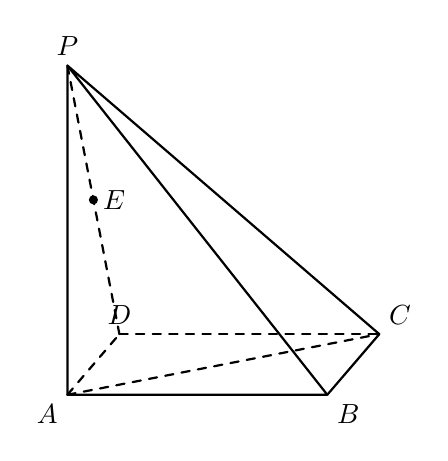
\begin{tikzpicture}[>=stealth,scale=1.1,line cap=round,line join=round]
  % 顶点坐标
  \coordinate (A) at (0,0);
  \coordinate (B) at (3.0,0);
  \coordinate (D) at (0.6,0.7);
  \coordinate (C) at (3.6,0.7);
  \coordinate (P) at (0,3.8);
  \coordinate (E) at (0.3,2.25);

  % 虚线不可见棱与对角线
  \draw[dashed,thick] (A) -- (D);
  \draw[dashed,thick] (D) -- (C);
  \draw[dashed,thick] (P) -- (D);
  \draw[dashed,thick] (A) -- (C);

  % 实线可见棱
  \draw[thick] (P) -- (A) -- (B) -- (C) -- (P) -- (B);

  % 中点 E 绘制
  \fill (E) circle (1.5pt) node[right] {$E$};

  % 顶点标签
  \node[above] at (P) {$P$};
  \node[below left] at (A) {$A$};
  \node[below right] at (B) {$B$};
  \node[above right] at (C) {$C$};
  \node[above] at (D) {$D$};
\end{tikzpicture}
\end{center}
\nopagebreak[4]
(1) 求直线 $AC$ 与 $PB$ 所成角的余弦值；

(2) 在侧面 $PAB$ 内找一点 $N$，使 $NE \perp$ 面 $PAC$，并求出 $N$ 点到 $AB$ 和 $AP$ 的距离．

\Needspace{4\baselineskip}
\textbf{解析}

以点 $A$ 为原点，以直线 $AB, AD, AP$ 分别为 $x$ 轴、$y$ 轴、$z$ 轴正方向建立空间直角坐标系．
\Needspace{5\baselineskip}
依题意，$AB = \sqrt{3}, BC = AD = 1, PA = 2$，故各点坐标分别为：
\nopagebreak[4]
\[
A(0, 0, 0), \quad B(\sqrt{3}, 0, 0), \quad C(\sqrt{3}, 1, 0), \quad D(0, 1, 0), \quad P(0, 0, 2).
\]
\Needspace{5\baselineskip}
因为 $E$ 为 $PD$ 的中点，所以：
\nopagebreak[4]
\[
E\left(0, \frac{1}{2}, 1\right).
\]

\textbf{(1)}

\Needspace{5\baselineskip}
直线 $AC$ 与 $PB$ 的方向向量分别为：
\nopagebreak[4]
\[
\vec{AC} = (\sqrt{3}, 1, 0), \quad \vec{PB} = (\sqrt{3}, 0, -2).
\]
\Needspace{5\baselineskip}
其模长为：
\nopagebreak[4]
\[
|\vec{AC}| = \sqrt{(\sqrt{3})^2 + 1^2 + 0^2} = 2, \quad |\vec{PB}| = \sqrt{(\sqrt{3})^2 + 0^2 + (-2)^2} = \sqrt{7}.
\]
\Needspace{5\baselineskip}
两向量的数量积为：
\nopagebreak[4]
\[
\vec{AC} \cdot \vec{PB} = \sqrt{3} \times \sqrt{3} + 1 \times 0 + 0 \times (-2) = 3.
\]
\Needspace{5\baselineskip}
设直线 $AC$ 与 $PB$ 所成的角为 $\theta$，则：
\nopagebreak[4]
\[
\cos\theta = \frac{|\vec{AC} \cdot \vec{PB}|}{|\vec{AC}||\vec{PB}|} = \frac{3}{2 \times \sqrt{7}} = \frac{3\sqrt{7}}{14}.
\]
故直线 $AC$ 与 $PB$ 所成角的余弦值为 $\dfrac{3\sqrt{7}}{14}$．

\textbf{(2)}

侧面 $PAB$ 位于 $xOz$ 平面内（即方程为 $y = 0$）．
\Needspace{5\baselineskip}
设点 $N$ 的坐标为 $(x_0, 0, z_0)$，则：
\nopagebreak[4]
\[
\vec{NE} = \left(-x_0, \frac{1}{2}, 1 - z_0\right).
\]
平面 $PAC$ 包含直线 $AP$ 与 $AC$，其方向向量分别为 $\vec{AP} = (0, 0, 2)$ 与 $\vec{AC} = (\sqrt{3}, 1, 0)$．
要使 $NE \perp$ 面 $PAC$，只需 $\vec{NE} \perp \vec{AP}$ 且 $\vec{NE} \perp \vec{AC}$：
\begin{itemize}
\item 由 $\vec{NE} \cdot \vec{AP} = 0$ 得：
\end{itemize}
\nopagebreak[4]
\[
2(1 - z_0) = 0 \implies z_0 = 1;
\]
\begin{itemize}
\item 由 $\vec{NE} \cdot \vec{AC} = 0$ 得：
\end{itemize}
\nopagebreak[4]
\[
-\sqrt{3}x_0 + \frac{1}{2} \times 1 = 0 \implies x_0 = \frac{1}{2\sqrt{3}} = \frac{\sqrt{3}}{6}.
\]

因此点 $N$ 的坐标为 $\left(\dfrac{\sqrt{3}}{6}, 0, 1\right)$．
在平面 $PAB$ 内，直线 $AB$ 即为 $x$ 轴（$z = 0$），直线 $AP$ 即为 $z$ 轴（$x = 0$）．
所以：
\begin{itemize}
\item 点 $N$ 到 $AB$ 的距离为 $|z_0| = 1$；
\item 点 $N$ 到 $AP$ 的距离为 $|x_0| = \dfrac{\sqrt{3}}{6}$．
\end{itemize}

\gkanswer{答案（1）：直线 $AC$ 与 $PB$ 所成角的余弦值为 $\dfrac{3\sqrt{7}}{14}$。}

\gkanswer{答案（2）：$N$ 点到 $AB$ 的距离为 $1$，$N$ 点到 $AP$ 的距离为 $\dfrac{\sqrt{3}}{6}$。}

\end{answer}
\begin{answer}
\gksolhead{21}{}

\textbf{题目}：

（本小题满分 12 分）

设 $A, B$ 是椭圆 $3x^2 + y^2 = \lambda$ 上的两点，点 $N(1, 3)$ 是线段 $AB$ 的中点，线段 $AB$ 的垂直平分线与椭圆相交于 $C, D$ 两点．

(1) 确定 $\lambda$ 的取值范围，并求直线 $AB$ 的方程；

(2) 试判断是否存在这样的 $\lambda$，使得 $A, B, C, D$ 四点在同一个圆上？并说明理由．

\Needspace{4\baselineskip}
\textbf{解析}

\textbf{(1)}

设 $A(x_1, y_1), B(x_2, y_2)$ 为椭圆 $3x^2 + y^2 = \lambda$ 上的相异两点．
\Needspace{5\baselineskip}
因为点 $N(1, 3)$ 是线段 $AB$ 的中点，点 $N$ 必位于椭圆内部，因此：
\nopagebreak[4]
\[
3 \times 1^2 + 3^2 < \lambda \iff 3 + 9 < \lambda \iff \lambda > 12.
\]
\Needspace{5\baselineskip}
两点坐标代入椭圆方程得：
\nopagebreak[4]
\[
3x_1^2 + y_1^2 = \lambda, \quad 3x_2^2 + y_2^2 = \lambda.
\]
\Needspace{5\baselineskip}
两式相减可得：
\nopagebreak[4]
\[
3(x_1 - x_2)(x_1 + x_2) + (y_1 - y_2)(y_1 + y_2) = 0.
\]
因为 $N(1, 3)$ 为 $AB$ 的中点，所以 $x_1 + x_2 = 2$，$y_1 + y_2 = 6$．
\Needspace{5\baselineskip}
代入上式得：
\nopagebreak[4]
\[
3(x_1 - x_2) \times 2 + (y_1 - y_2) \times 6 = 0 \implies 6(x_1 - x_2) + 6(y_1 - y_2) = 0.
\]
\Needspace{5\baselineskip}
因为 $A, B$ 是相异两点，所以 $x_1 \neq x_2$．两边同除以 $6(x_1 - x_2)$ 得直线 $AB$ 的斜率：
\nopagebreak[4]
\[
k_{AB} = \frac{y_1 - y_2}{x_1 - x_2} = -1.
\]
\Needspace{5\baselineskip}
所以直线 $AB$ 的方程为：
\nopagebreak[4]
\[
y - 3 = -(x - 1) \iff x + y - 4 = 0.
\]
\Needspace{5\baselineskip}
联立直线 $AB$ 与椭圆方程检验交点：将 $y = 4 - x$ 代入 $3x^2 + y^2 = \lambda$ 得：
\nopagebreak[4]
\[
3x^2 + (4 - x)^2 = \lambda \iff 4x^2 - 8x + 16 - \lambda = 0.
\]
\Needspace{5\baselineskip}
判别式为：
\nopagebreak[4]
\[
\Delta = (-8)^2 - 4 \times 4(16 - \lambda) = 16(\lambda - 12).
\]
当 $\lambda > 12$ 时，$\Delta > 0$ 恒成立，方程有两个相异实根，直线与椭圆确实有两个交点．
故 $\lambda$ 的取值范围是 $(12, +\infty)$，直线 $AB$ 的方程为 $x + y - 4 = 0$．

\textbf{(2)}

存在满足条件的 $\lambda$．事实上，对任意 $\lambda \in (12, +\infty)$，$A, B, C, D$ 四点恒在同一个圆上．
证明如下：
由题意，线段 $AB$ 的垂直平分线即为直线 $CD$．
因为直线 $AB$ 的斜率为 $-1$，所以直线 $CD$ 的斜率为 $k_{CD} = -\dfrac{1}{k_{AB}} = 1$．
\Needspace{5\baselineskip}
又直线 $CD$ 过点 $N(1, 3)$，故其方程为：
\nopagebreak[4]
\[
y - 3 = 1 \times (x - 1) \iff y = x + 2.
\]
\Needspace{5\baselineskip}
因为弦 $AB$ 与弦 $CD$ 垂直相交于点 $N(1, 3)$，根据相交弦定理的逆定理，四点 $A, B, C, D$ 共圆的充要条件为：
\nopagebreak[4]
\[
|NA| \cdot |NB| = |NC| \cdot |ND|.
\]
利用直线的参数方程求弦长积：
\begin{itemize}
\item 设直线 $AB$ 的参数方程为（以 $N(1, 3)$ 为基点，倾斜角为 $\dfrac{3\pi}{4}$）：
\end{itemize}
\nopagebreak[4]
\[
\begin{cases}
x = 1 - \dfrac{\sqrt{2}}{2}t, \\
y = 3 + \dfrac{\sqrt{2}}{2}t
\end{cases}
\]
\Needspace{5\baselineskip}
  代入椭圆方程 $3x^2 + y^2 = \lambda$：
\nopagebreak[4]
\[
3\left(1 - \frac{\sqrt{2}}{2}t\right)^2 + \left(3 + \frac{\sqrt{2}}{2}t\right)^2 = \lambda.
\]
\Needspace{5\baselineskip}
  展开化简：
\nopagebreak[4]
\[
3\left(1 - \sqrt{2}t + \frac{1}{2}t^2\right) + \left(9 + 3\sqrt{2}t + \frac{1}{2}t^2\right) = \lambda \implies 2t^2 + 12 = \lambda.
\]
\Needspace{5\baselineskip}
  设 $A, B$ 对应的参数为 $t_1, t_2$，则 $t^2 = \dfrac{\lambda - 12}{2}$，从而：
\nopagebreak[4]
\[
|NA| \cdot |NB| = |t_1 t_2| = \frac{\lambda - 12}{2};
\]
\begin{itemize}
\item 设直线 $CD$ 的参数方程为（以 $N(1, 3)$ 为基点，倾斜角为 $\dfrac{\pi}{4}$）：
\end{itemize}
\nopagebreak[4]
\[
\begin{cases}
x = 1 + \dfrac{\sqrt{2}}{2}s, \\
y = 3 + \dfrac{\sqrt{2}}{2}s
\end{cases}
\]
\Needspace{5\baselineskip}
  代入椭圆方程 $3x^2 + y^2 = \lambda$：
\nopagebreak[4]
\[
3\left(1 + \frac{\sqrt{2}}{2}s\right)^2 + \left(3 + \frac{\sqrt{2}}{2}s\right)^2 = \lambda.
\]
\Needspace{5\baselineskip}
  展开化简：
\nopagebreak[4]
\[
3\left(1 + \sqrt{2}s + \frac{1}{2}s^2\right) + \left(9 + 3\sqrt{2}s + \frac{1}{2}s^2\right) = \lambda \implies 2s^2 + 6\sqrt{2}s + 12 - \lambda = 0.
\]
\Needspace{5\baselineskip}
  设 $C, D$ 对应的参数为 $s_1, s_2$，由韦达定理：
\nopagebreak[4]
\[
s_1 s_2 = \frac{12 - \lambda}{2} = -\frac{\lambda - 12}{2}.
\]
\Needspace{5\baselineskip}
  从而：
\nopagebreak[4]
\[
|NC| \cdot |ND| = |s_1 s_2| = \left|-\frac{\lambda - 12}{2}\right| = \frac{\lambda - 12}{2}.
\]

\Needspace{5\baselineskip}
比较两式可知，恒有：
\nopagebreak[4]
\[
|NA| \cdot |NB| = |NC| \cdot |ND| = \frac{\lambda - 12}{2}.
\]
由相交弦定理的逆定理，$A, B, C, D$ 四点恒在同一个圆上．
因此，存在满足题意的 $\lambda$，且任意 $\lambda \in (12, +\infty)$ 均使得 $A, B, C, D$ 四点在同一个圆上．

\gkanswer{答案（1）：$\lambda$ 的取值范围是 $(12, +\infty)$；直线 $AB$ 的方程为 $x + y - 4 = 0$。}

\gkanswer{答案（2）：存在，四点 $A, B, C, D$ 对任意 $\lambda \in (12, +\infty)$ 恒共圆，证明见解析。}

\end{answer}
\begin{answer}
\gksolhead{22}{}

\textbf{题目}：

（本小题满分 14 分）

已知不等式 $\dfrac{1}{2} + \dfrac{1}{3} + \dots + \dfrac{1}{n} > \dfrac{1}{2}[\log_2 n]$，其中 $n$ 为大于 2 的整数，$[\log_2 n]$ 表示不超过 $\log_2 n$ 的最大整数．设数列 $\{a_n\}$ 的各项为正，且满足 $a_1 = b$ ($b > 0$)，$a_n \leqslant \dfrac{n a_{n-1}}{n + a_{n-1}}$ ($n = 2, 3, 4, \dots$)．

(1) 证明：$a_n < \dfrac{2b}{2 + b[\log_2 n]}$ ($n = 3, 4, 5, \dots$)；

(2) 猜测数列 $\{a_n\}$ 是否有极限？如果有，写出极限的值（不必证明）；

(3) 试确定一个正整数 $N$，使得当 $n > N$ 时，对任意 $b > 0$，都有 $a_n < \dfrac{1}{5}$．

\Needspace{4\baselineskip}
\textbf{解析}

\textbf{(1)}

\Needspace{5\baselineskip}
因为数列 $\{a_n\}$ 的各项均为正数，对递推不等式两边取倒数：
\nopagebreak[4]
\[
\frac{1}{a_n} \geqslant \frac{n + a_{n-1}}{n a_{n-1}} = \frac{1}{a_{n-1}} + \frac{1}{n} \quad (n = 2, 3, 4, \dots).
\]
\Needspace{5\baselineskip}
由此递推累加可得：
\nopagebreak[4]
\[
\frac{1}{a_2} \geqslant \frac{1}{a_1} + \frac{1}{2} = \frac{1}{b} + \frac{1}{2},
\]
\nopagebreak[4]
\[
\frac{1}{a_3} \geqslant \frac{1}{a_2} + \frac{1}{3} \geqslant \frac{1}{b} + \frac{1}{2} + \frac{1}{3},
\]
\Needspace{5\baselineskip}
一般地，当 $n \geqslant 3$ 时：
\nopagebreak[4]
\[
\frac{1}{a_n} \geqslant \frac{1}{b} + \sum_{k=2}^n \frac{1}{k} = \frac{1}{b} + \left(\frac{1}{2} + \frac{1}{3} + \dots + \frac{1}{n}\right).
\]
\Needspace{5\baselineskip}
利用题设已知不等式 $\dfrac{1}{2} + \dfrac{1}{3} + \dots + \dfrac{1}{n} > \dfrac{1}{2}[\log_2 n]$，得：
\nopagebreak[4]
\[
\frac{1}{a_n} > \frac{1}{b} + \frac{1}{2}[\log_2 n] = \frac{2 + b[\log_2 n]}{2b}.
\]
\Needspace{5\baselineskip}
因为 $b > 0$ 且各项为正，不等式两边皆为正实数，两边取倒数改变不等号方向：
\nopagebreak[4]
\[
a_n < \frac{2b}{2 + b[\log_2 n]} \quad (n = 3, 4, 5, \dots).
\]
原命题获证．

\textbf{(2)}

猜测数列 $\{a_n\}$ 存在极限，且极限值为 0．
\Needspace{5\baselineskip}
理由如下：由 (1) 知，对 $n \geqslant 3$ 恒有：
\nopagebreak[4]
\[
0 < a_n < \frac{2b}{2 + b[\log_2 n]} = \frac{2}{\dfrac{2}{b} + [\log_2 n]}.
\]
当 $n \to \infty$ 时，$\log_2 n \to +\infty$，故 $[\log_2 n] \to +\infty$．
\Needspace{5\baselineskip}
因此：
\nopagebreak[4]
\[
\lim_{n\to\infty} \frac{2}{\dfrac{2}{b} + [\log_2 n]} = 0.
\]
\Needspace{5\baselineskip}
由夹逼定理可知：
\nopagebreak[4]
\[
\lim_{n\to\infty} a_n = 0.
\]

\textbf{(3)}

\Needspace{5\baselineskip}
由 (1) 的结论，对任意 $n \geqslant 3$ 及任意 $b > 0$：
\nopagebreak[4]
\[
a_n < \frac{2b}{2 + b[\log_2 n]} = \frac{2}{\dfrac{2}{b} + [\log_2 n]}.
\]
\Needspace{5\baselineskip}
因为 $b > 0$，所以 $\dfrac{2}{b} > 0$，从而：
\nopagebreak[4]
\[
\frac{2}{\dfrac{2}{b} + [\log_2 n]} < \frac{2}{[\log_2 n]}.
\]
\Needspace{5\baselineskip}
要使对任意 $b > 0$ 均有 $a_n < \dfrac{1}{5}$，只需满足：
\nopagebreak[4]
\[
\frac{2}{[\log_2 n]} \leqslant \frac{1}{5} \iff [\log_2 n] \geqslant 10.
\]
\Needspace{5\baselineskip}
因为函数 $[\log_2 n]$ 关于正整数 $n$ 单调不减，且：
\nopagebreak[4]
\[
[\log_2 n] \geqslant 10 \iff \log_2 n \geqslant 10 \iff n \geqslant 2^{10} = 1024.
\]
所以取正整数 $N = 1023$（或取大于等于 1023 的任意正整数，如 1023）．
当 $n > N = 1023$ 时，必有 $n \geqslant 1024$，此时 $[\log_2 n] \geqslant 10$．
\Needspace{5\baselineskip}
对任意 $b > 0$，恒有：
\nopagebreak[4]
\[
a_n < \frac{2}{\dfrac{2}{b} + [\log_2 n]} < \frac{2}{[\log_2 n]} \leqslant \frac{2}{10} = \frac{1}{5}.
\]
因此，正整数 $N$ 可取为 1023．

\gkanswer{答案（1）：证明见解析。}

\gkanswer{答案（2）：数列 $\{a_n\}$ 存在极限，且 $\lim_{n\to\infty} a_n = 0$。}

\gkanswer{答案（3）：取正整数 $N = 1023$（或取满足 $N \geqslant 1023$ 的任意正整数），当 $n > N$ 时，对任意 $b > 0$ 恒有 $a_n < \dfrac{1}{5}$。}

\end{answer}